\documentclass[a4paper, 12pt]{article}
\usepackage{geometry}
\geometry{a4paper,
total={170mm,257mm},left=2cm,right=2cm,
top=2cm,bottom=2cm}

\usepackage{mathtext}
\usepackage{amssymb}
\usepackage{amsmath}
\usepackage{multirow}
\usepackage[T2A]{fontenc}
\usepackage[utf8]{inputenc}
\usepackage[english, russian]{babel}
\usepackage{graphicx, float}
\usepackage{tabularx, colortbl}
\usepackage{caption}
\captionsetup{labelsep=period}

\newcommand{\parag}[1]{\paragraph*{#1:}}
\DeclareSymbolFont{T2Aletters}{T2A}{cmr}{m}{it}
\newcounter{Points}
\setcounter{Points}{1}
\newcommand{\point}{\arabic{Points}. \addtocounter{Points}{1}}
\newcolumntype{C}{>{\centering\arraybackslash}X}

\author{Калинин Даниил, Б01-110}
\date{\today}
\title{Лабораторная работа 2.1.4\\Определение коэффициента теплопроводности твердых тел}

\begin{document}
\maketitle

\parag {Цель работы}
определенить коэффициенты теплопроводности твердых тел путем сравнения с теплопроводностью эталонного материала; вычислить относительные тепловые потери через боковые поверхности по измеренным значениям температуры вдоль радиусов пластинок.
	
\parag {В работе используются}
термостат, набор из четырех термопар, гальванометр, резиновые прокладки, диски из исследуемых материалов, диск из эталонного материала (эбонита), штангенциркуль.

\parag {Теоритическая справка} ~\\

Количество теплоты $\Delta q$, протекающее за единицу времени через однородную перегородку толщиной $\Delta z$ и площадью $S$ при разности температур $\Delta T$, определяется формулой

\begin{equation}
    \label{delta_q}
    \Delta q = \varkappa S \frac{\Delta T}{\Delta z},
\end{equation}

где $ \varkappa $ -- коэффициент теплопроводности, характеризующий свойства материала.

Значение коэффициента теплопроводности $\varkappa$ может быть определено непосредственно из формулы \eqref{delta_q}, если измерить на опыте все параметры из данной формулы. Однако такой подход вызывает трудности, связанные с точным измерением количества теплоты $\Delta q$. Поэтому в нашей работе вместо измерения величины $\varkappa$, произведём сравнение теплопроводности исследуемого материала с теплопроводностью некоторого другого эталонного материала с хорошо известным значением данного коэффициента. Таким образом можно избежать измерения $\Delta q$.

В нашем методе две пластинки, изготовленные из материалов с коэффициентами теплопроводности $\varkappa_{1}$ и $\varkappa_{2}$, зажимаются между стенками, температуры которых равны $T_1$ и $T_2$ и поддерживаются постоянными во время опыта. Если толщины пластинок $d_{1}$ и $d_{2}$ достаточно малы (по сравнению с наименьшим линейным размером их поверхности), то и потери тепла через боковые поверхности тоже малы. В таком случае площадь теплового потока, протекающего от горячей стенки к холодной, приблизительно остается постоянной. В этом случае

\begin{equation}
    \label{delta_q_experimental}
    \Delta q = \varkappa_{1} S \frac{\Delta T_1}{\Delta z_1} = \varkappa_2 S \frac{\Delta T_2}{\Delta z_2}.
\end{equation}

Полагая, что $ \Delta z_1 = d_1 $ и $ \Delta z_2 = d_2 $, получим окончательно

\begin{equation}
    \label{final_formula}
    \frac{\varkappa_1}{\varkappa_2} = \frac{d_1}{d_2}\frac{\Delta T_2}{\Delta T_1},
\end{equation}

где $ \Delta T_1 $ и $ \Delta T_2 $ -- перепады температур на пластинках. Зная теплопроводность материала одной из пластинок, легко определить на опыте теплопроводность другой пластинки.

Чтобы оценить размер тепловых потерь через боковые стороны исследуемого образца, нужно определить плотность радиального потока тепла $q_r$. Эта величина определяется радиальным значением градиента температуры. Полный радиальный поток есть произведение $q_r$ и площади боковой поверхности $S_r$, вычисленной на том же расстоянии от оси симметрии, на котором производилось измерение радиальной производной температуры

\begin{equation}
    \label{losses_1}
    q_r S_r = - \varkappa 2 \pi rd \frac{\partial T}{\partial r},
\end{equation}
где d -- толщина пластины.

Полный осевой поток определяется произведением производной температуры вдоль оси симметрии $z$ и площади окружности, проходящей через точку измерения радиальной производной:

\begin{equation}
    \label{losses_2}
    q_z S_z = - \varkappa \pi r^2 \frac{\partial T}{\partial z}.
\end{equation}

Отношение этих потоков обозначим $ \delta $:

\begin{equation}
    \label{losses_3}
    \delta = \frac{2d \frac{\partial T}{\partial r}}{r \frac{\partial T}{\partial z}}.
\end{equation}

Этот параметр характеризует расширение теплового потока и его относительные потери, он не зависит от коэффициента теплопроводности.

\parag{Экспериментальная установка}

\begin{figure}[H]
	\begin{center}
		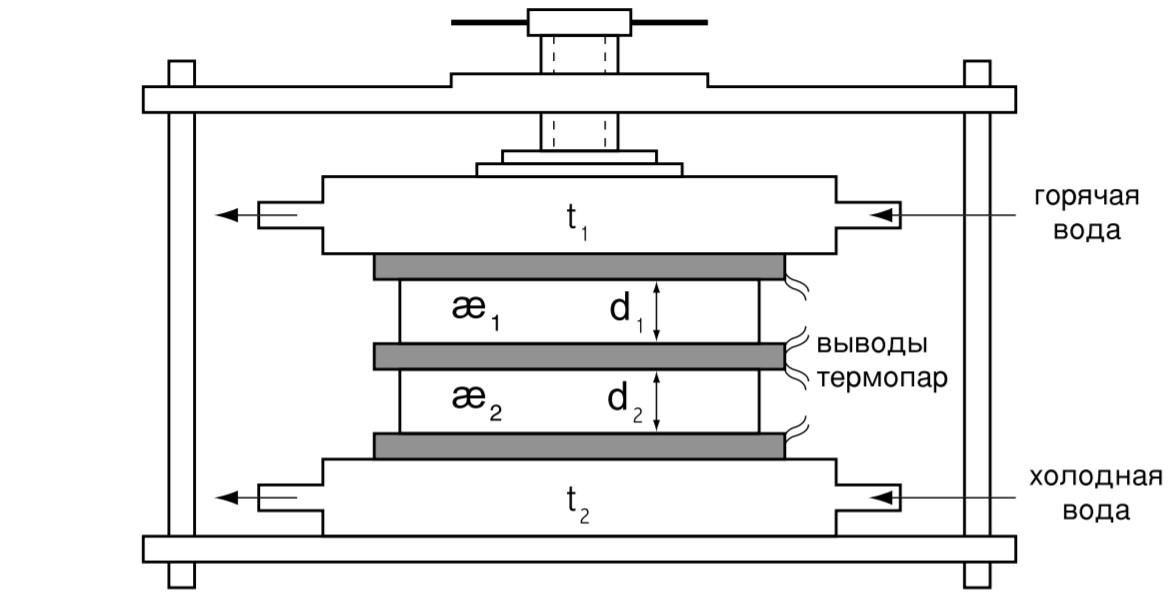
\includegraphics[width=15cm]{setup.jpg}
		\caption{Чертеж экспериментальной установки}
        \label{img:setup}
	\end{center}
\end{figure}

На рисунке \ref{img:setup} изображен прибор для измерения коэффициента теплопроводности. Он представляет собой систему из нагревателя, имеющего температуру $ T_1 $, и холодильника, имеющего температуру $ T_2 $; эти температуры поддерживаются постоянными. Тепловой поток от нагревателя к холодильнику протекает через зажатые между ними пластинки из исследуемого и эталонного материала. 

В нашем приборе эталонным материалом является эбонит, коэффициент теплопроводности которого равен $ 0,18~\frac{Вт}{м \cdot К}$. Для получения надежного теплового контакта между поверхностями прокладывается резина. 

При измерениях коэффициента теплопроводности между нагревателем и холодильником закладываются переложенные тонкими резиновыми прокладками пластинки из исследуемого и эталонного материалов. Вся система сжимается винтовым прессом. 

Для стабилизации температур $ T_1 $ и $ T_2 $ через холодильник постоянно пропускается проточная вода из водопровода, а через нагреватель циркулирует горячая вода, поставляемая термостатом. Измерение температур производится при помощи четырех термопар.

\parag {Ход работы} ~\\
\point Перед началом работы, расчитаем время установления теплового равновесия. Сделать это можно по формуле:
$$d^2 = \chi \cdot t$$
Для эбонита, $\chi = 6 \cdot 10^{-6}~м^2/c, d = 3.84 мм$, тогда 
$$t_{равновесия} \approx 246~c.$$

\point Теперь откалибруем термопары. Расположим все 4 термопары близко к центру эбонитовой пластинки, расположенной в установке. Дождемся установления теплового равновесия и снимем показания гальванометра. Резульаты занесем в таблицу \ref{tabl:calibration}.

\begin{table}[h]
    \centering
    \begin{tabular}{|l|l|}
    \hline 
    Номер термопары & Показание гальванометра       \\ \hline
    1               & 0.20                          \\ \hline    
    2               & 0.20                          \\ \hline    
    3               & 0.21                          \\ \hline    
    4               & 0.21                          \\ \hline    
    \end{tabular}
	\caption{Данные калибровки термопар}
    \label{tabl:calibration}
\end{table}

Из таблицы \ref{tabl:calibration} видно, что показания почти не отличаются, тем не менее, для наибольшей точности, при расчетах отношения температур, будем пользоваться следющей формулой:
\begin{equation}
    \label{temperature_ratio}
    \frac{\Delta T_1}{\Delta T_2} = \frac{U_2/\alpha_2-U_1/\alpha_1}{U_4/\alpha_4-U_3/\alpha_3},
\end{equation}

где $U_1,~U_2,~U_3,~U_4$ -- показания гальванометра, полученные во время опыта, $alpha_1,~alpha_2,~alpha_3,~alpha_4$ -- показания из таблицы \ref{tabl:calibration}, соответственно.

\point Следющим шагом, проверим, что коэффициент теплопроводности эбонита не зависит от температур в рабочем диапазоне. Для этого поместим в установку две пластины эбонита. Измерим разности температур на пластинах. Занесем результаты в таблицу \ref{tabl:ebo-ebo}
\begin{table}[h]
    \centering
    \begin{tabular}{|l|l|}
    \hline 
    Номер термопары & Показание гальванометра       \\ \hline
    1               & 0.17                          \\ \hline    
    2               & 0.84                          \\ \hline    
    3               & 0.86                          \\ \hline    
    4               & 1.63                          \\ \hline    
    \end{tabular}
	\caption{Данные измерений в системе эбонит-эбонит}
    \label{tabl:ebo-ebo}
\end{table}

Из формулы \ref{temperature_ratio} получим:
$$ \frac{\Delta T_{12}}{\Delta T_{34}} = 0.913 \approx \frac{d_1}{d_2}$$
Равенство выше подтвержает верность гипотезы о том, что теплопроводность эбонита не зависит от температуры, по крайней мере в том диапазоне температур, в котором мы работаем.

\point Перейдем к основной части эксперимента. Определим теплопроводности плексигласа, текстолита, стекло-текстолита. Для надежности, проведем каждый опыт дважды: в первом случае исследуемый элемент будет ближе к холодильнику, во втором -- к нагревателю. Результаты измерений занесем в таблицы \ref{tabl:0}, \ref{tabl:1}, \ref{tabl:2}.

\begin{table}[h]
    \centering
    \begin{tabular}{|c|c|c|c|c|}
    
    \hline
    №	&	\multicolumn{2}{c}{Температура,	у.е.}	&	Название	материала	&	d,	мм.	\\\hline
    
    1	&	0.1	&	0.15	&	
    &	\\\cline{1-3}
    2	&	0.81	&	1.07	&	
    \multirow{3}{*}{\textbf{Плексигласс}}	&	\multirow{3}{*}{4.74	$\pm	0.05$}	\\\cline{1-3}
    
    3	&	0.87	&	1	&	
    &	\\\cline{1-3}
    4	&	2	&	2	&	
    &	\\\cline{1-3}
        &	\textbf{холодильник}	&	\textbf{нагреватель}	&	&
    \\\hline
    \end{tabular}
    
    \caption{Таблица с данными измерения для материала плексигласс}
    \label{tabl:0}
    \end{table}
    \begin{table}[h]
    \centering
    \begin{tabular}{|c|c|c|c|c|}
    
    \hline
    №	&	\multicolumn{2}{c}{Температура,	у.е.}	&	Название	материала	&	d,	мм.	\\\hline
    
    1	&	0.12	&	0.18	&	
    &	\\\cline{1-3}
    2	&	1.13	&	0.92	&	
    \multirow{3}{*}{\textbf{Текстолит}}	&	\multirow{3}{*}{4.3	$\pm	0.05$}	\\\cline{1-3}
    
    3	&	1.08	&	0.91	&	
    &	\\\cline{1-3}
    4	&	1.98	&	1.97	&	
    &	\\\cline{1-3}
        &	\textbf{холодильник}	&	\textbf{нагреватель}	&	&
    \\\hline
    \end{tabular}
    
    \caption{Таблица с данными измерения для материала текстолит}
    \label{tabl:1}
    \end{table}
    \begin{table}[h]
    \centering
    \begin{tabular}{|c|c|c|c|c|}
    
    \hline
    №	&	\multicolumn{2}{c}{Температура,	у.е.}	&	Название	материала	&	d,	мм.	\\\hline
    
    1	&	0.15	&	0.22	&	
    &	\\\cline{1-3}
    2	&	1.28	&	0.96	&	
    \multirow{3}{*}{\textbf{Стекло-Текстолит}}	&	\multirow{3}{*}{1.6	$\pm	0.05$}	\\\cline{1-3}
    
    3	&	1.32	&	0.9	&	
    &	\\\cline{1-3}
    4	&	1.96	&	1.97	&	
    &	\\\cline{1-3}
        &	\textbf{холодильник}	&	\textbf{нагреватель}	&	&
    \\\hline
    \end{tabular}
    
    \caption{Таблица с данными измерения для материала стекло-текстолит}
    \label{tabl:2}
\end{table}

\point Из полученных данных, посчитаем $\varkappa$ для каждого из материалов. Результаты занесем в таблицу \ref{tabl:results}.

\begin{table}[h]
    \centering
    \begin{tabular}{|c|c|c|c|}
    \hline
    
    № & Материал & Метод измерения & $\varkappa,~\frac{Вт \cdot м}{K}$ \\ \hline
    \multirow{2}{*}{1} & \multirow{2}{*}{\textbf{Плексигласс}} & нагреватель  & 0.130 $\pm 0.019$ \\ \cline{3-4}
    & & холодильник  & 0.205 $\pm 0.019$ \\ \hline
    
    \multirow{2}{*}{2} & \multirow{2}{*}{\textbf{Текстолит}} &нагреватель  & 0.109 $\pm 0.009$ \\ \cline{3-4}
    & & холодильник  & 0.126 $\pm 0.009$ \\ \hline

    \multirow{2}{*}{3} & \multirow{2}{*}{\textbf{Стекло-Текстолит}} & нагреватель  & 0.290 $\pm 0.017$ \\ \cline{3-4}
    & & холодильник  & 0.216 $\pm 0.017$ \\ \hline
    
\end{tabular}

    \caption{Коэффициетны теплопроводности для разных материалов}
    \label{tabl:results}
\end{table}

В конечном итоге получаем:

\begin{itemize}
    \item плексиглас: $ \varkappa = 0.167 \pm 0.019~\frac{Вт}{м \cdot с} $, ($\varepsilon = 11.3\%$)
    
    \item текстолит: $ \varkappa = 0.118 \pm 0.008)~\frac{Вт}{м \cdot с} $, ($\varepsilon = 12.8\%$)
    
    \item стекло-текстолит: $ \varkappa = 0.253 \pm 0.017~\frac{Вт}{м \cdot с} $, ($\varepsilon = 7.88\%$)
\end{itemize}

\point Перейдем к финальной части работы.

Оценим потери через боковые поверхности. Разместим рабочие спаи термопар на разных расстояниях от центра пластины. Чтобы избежать ошибок, связанных с теплоотводом через провода термопар в этом точном эксперименте, длины всех прижатых частей проводов сделаем одинаковыми. С помощью гальванометра измерим температуры всех спаев и результаты измерений (делённые на соответствующую чувствительность) занесём в таблицу \ref{tab:losses}.

\begin{table}[H]
	\centering
	\begin{tabular}{|l|l|l|}
		\hline
		$ r $, мм & $ U $, у.е. & $ U/\alpha $  \\ \hline
		1,1   & 1,16    & 1,18 \\ \hline
		9,7   & 1,14    & 1,16 \\ \hline
		24,1  & 1,1     & 1,07 \\ \hline
		42,6  & 0,88    & 0,94 \\ \hline
	\end{tabular}
	\caption{Измерение распределения температур}
	\label{tab:losses}
\end{table}

Построим график зависимости от радиуса показаний гальванометра, поделенных на чувствительность каждой термопары (см. рис. \ref{img:gr2}). 

\begin{figure}[h]
	\begin{center}
		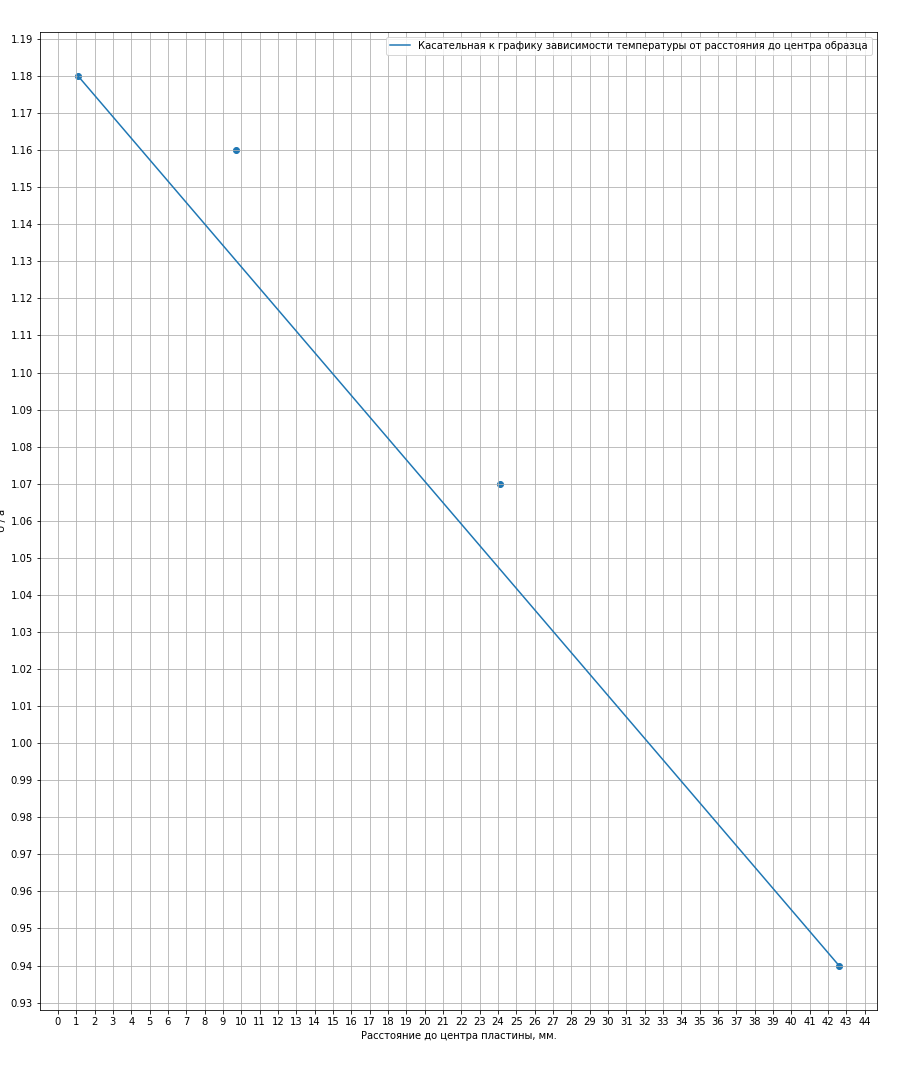
\includegraphics[width=18cm]{u_to_r.png}
		\caption{График зависимости температуры от расстояния до центра образца}\label{img:gr2}
	\end{center}
\end{figure}

Из графика получаем коэффициет наклона: $k = -0.0053 \approx 0.006$

Уменьшение температуры при удалении от центра обусловлено тепловым потоком через боковые поверхности. По графику найдём производную температуры по радиусу.

Так как распределение температуры по радиусы близко к параболическому, то производная в точке $ r = 42,6 $ мм в два раза больше производной для прямой, соединяющей температуру в этой точке с температурой в центре пластины.

Отсюда получаем \[ \frac{\partial T}{\partial r} = 2 \cdot (-0.006) = -0.012  у.е./мм. \]

Из опытов с эбонитовой пластинкой в прошлых экспериментах получаем, что

\[ \frac{\partial T}{\partial z} = 0.303  у.е./мм. \]

При этом радиус исследуемого образца равен $r = 50,4 $ мм, он был измерен при помощи штангенциркуля.

Тогда по формуле \eqref{losses_3} \[ \delta = \frac{2d \frac{\partial T}{\partial r}}{r \frac{\partial T}{\partial z}}  \approx 6.13 \cdot 10^{-3}. \]

Таким образом величина относительных потерь составляет $ \delta = 0.6 \%$, что подтверждает малось радиального теплового потока по сравнению с осевым.


\parag {Заключение} ~\\

\end{document}
